\documentclass[a4paper, 12pt]{article}

% Поддержка русского языка
\usepackage[english, russian]{babel}
\usepackage[T2A]{fontenc}
\usepackage[utf8]{inputenc}
\usepackage{indentfirst}
\usepackage{hyperref}
\usepackage{graphicx}
\usepackage{wrapfig}
\usepackage{sidecap}

\usepackage{amsmath, amsfonts, amssymb, amsthm, mathtools}

%% Оформление страницы
\usepackage{extsizes}     % Возможность сделать 14-й шрифт
\usepackage{geometry}     % Простой способ задавать поля
\usepackage{setspace}     % Интерлиньяж
\usepackage{enumitem}     % Настройка окружений itemize и enumerate
\setlist{leftmargin=25pt} % Отступы в itemize и enumerate

\geometry{top=25mm}    % Поля сверху страницы
\geometry{bottom=30mm} % Поля снизу страницы
\geometry{left=20mm}   % Поля слева страницы
\geometry{right=20mm}  % Поля справа страницы

\setlength\parindent{15pt}        % Устанавливает длину красной строки 15pt
\linespread{1.3}                  % Коэффициент межстрочного интервала
%\setlength{\parskip}{0.5em}      % Вертикальный интервал между абзацами
%\setcounter{secnumdepth}{0}      % Отключение нумерации разделов
%\setcounter{section}{-1}         % Нумерация секций с нуля
\usepackage{multicol}			  % Для текста в нескольких колонках
\usepackage{soulutf8}             % Модификаторы начертания

% Титульный лист
\newcommand{\ProjectName}{Луна-9}
\newcommand{\FullProjectName}{Луна-9}

\usepackage{titleps}
\newpagestyle{main}{
	\setheadrule{0.1pt}
	\sethead{Проект по ВвАРКТ <<\ProjectName>>}{}{}
	\setfootrule{0.1pt}
	\setfoot{ПМИ МАИ, 2022}{}{\thepage}
}
\pagestyle{main}

\begin{document}
\begin{center}
	\huge{Проект по ВвАРКТ <<Луна-9>>} \\
	\large{(Первое в истории мягкое прилунение)} \\
	\Large{Project Research Document}\\
	\large{\textbf{Медведев Е.А}, Медведев Н.А, Кабанов А.А, Новиков Н.С, Мунтяну А.В} \\
	\large{(команда <<Луна-9>> / М8О-101Б-22)}
	\rule{\textwidth}{0.1pt}
\end{center}

\section*{Введение}
Изучение космоса всегда привлекало внимание большого количества людей по всему миру. 
\paragraph{Цель} Провести симуляцию миссии <<Луна-9>> в KSP, научиться работе с библиотекой KRPC, написать программу, получающие данные о полете во время симуляции в KSP, сравнить результаты работы программы с результатами, полученными с помощью математиечской и физической моделей.
\subsubsection*{Задачи}
\begin{enumerate}
	\item изучить доступную информацию о полете <<Луна-9>>;
	\item проанализировать ее;
	\item произвести расчеты и создать математическую и физическую модели;
	\item осуществить сборку аналогичной ракеты в KSP;
	\item запрограммировать функции подсчета основных параметров ракеты и ее полета;
	\item реализовать миссию в KSP:
	\begin{enumerate}
		\item вывести ракету на орбиту Земли;
		\item выход с орбиты Земли;
		\item преодолеть расстояние между Землей и Луной;
		\item выход на орбиту Луны;
		\item мягкая посадка на Луну;
	\end{enumerate}
	\item сравнить показания собственных функций с действительными.
\end{enumerate}


\section{Описание миссии}
\subsection{Описание миссии и исторические справки}
\begin{wrapfigure}{r}{0.3\textwidth} %this figure will be at the right
	\centering
	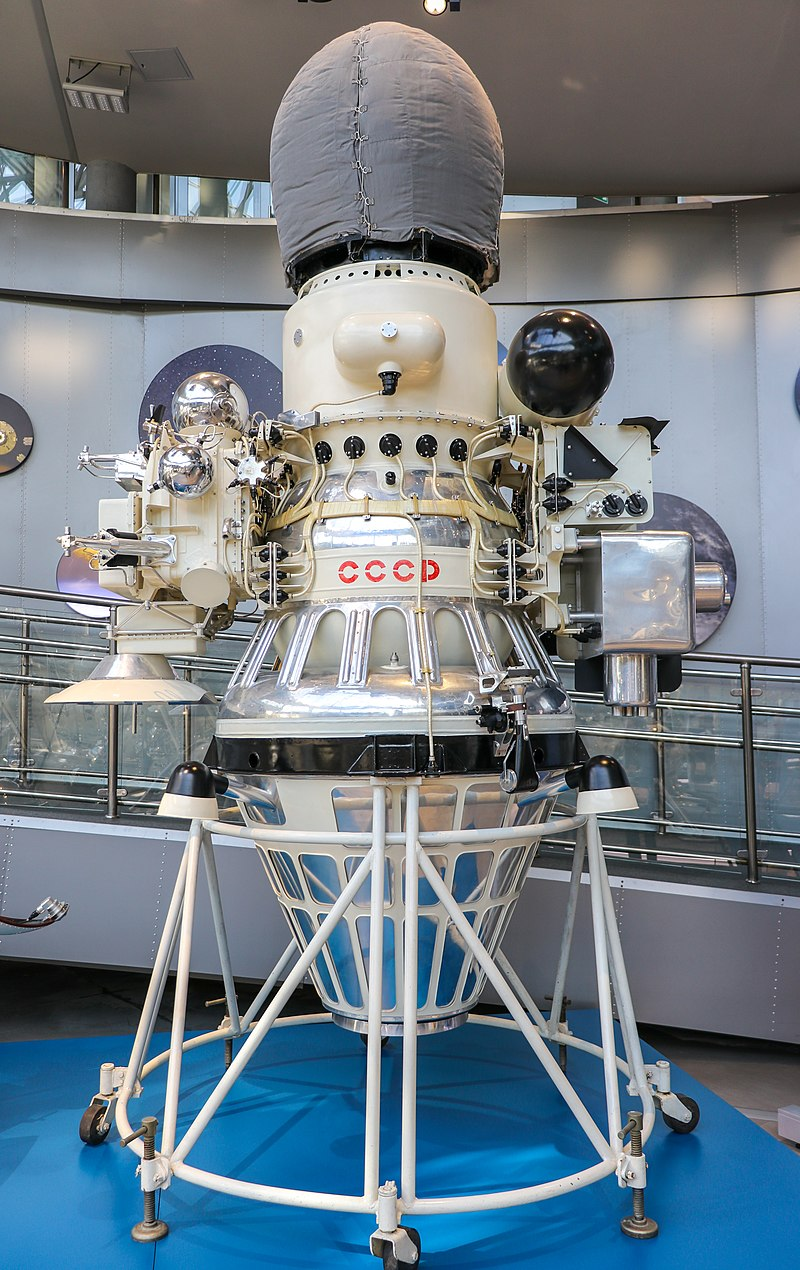
\includegraphics[width=0.3\textwidth]{Luna_9_Space_Probe}
	\caption{Модель межпланетной станции в Музее истории космонавтики имени К. Э. Циолковского}
\end{wrapfigure}

\noindent «Луна-9» — советская автоматическая межпланетная станция для изучения Луны и космического пространства. 

\noindent До неё было совершено одиннадцать попыток мягкой посадки на Луну по программе создания автоматических лунных станций типа Е-6. Только три аппарата достигли поверхности Луны, но разбились: «Луна-5», «Луна-7» и «Луна-8».

\noindent При реализации проекта были решены такие задачи, как запуск космических аппаратов в дальний космос с промежуточной околоземной орбиты, использование автономной астроориентации, коррекция траектории полета на большом удалении от Земли, осуществление прецизионного прицеливания и мягкая посадка на небесное тело, лишенное атмосферы.

\noindent Основным научным прибором, который планировалось доставить на Луну, была панорамная телевизионная камера. Кроме того, на борту станции находились приборы для регистрации космического излучения.

\noindent Ракета-носитель 8К78М («Молния») с аппаратом Е-6М стартовала 31 января 1966 года. Cтанция с разгонным блоком вышла на опорную орбиту, а затем вывела автоматическую станцию на заданную траекторию.

\begin{wrapfigure}{l}{0.4\textwidth}
	\centering
	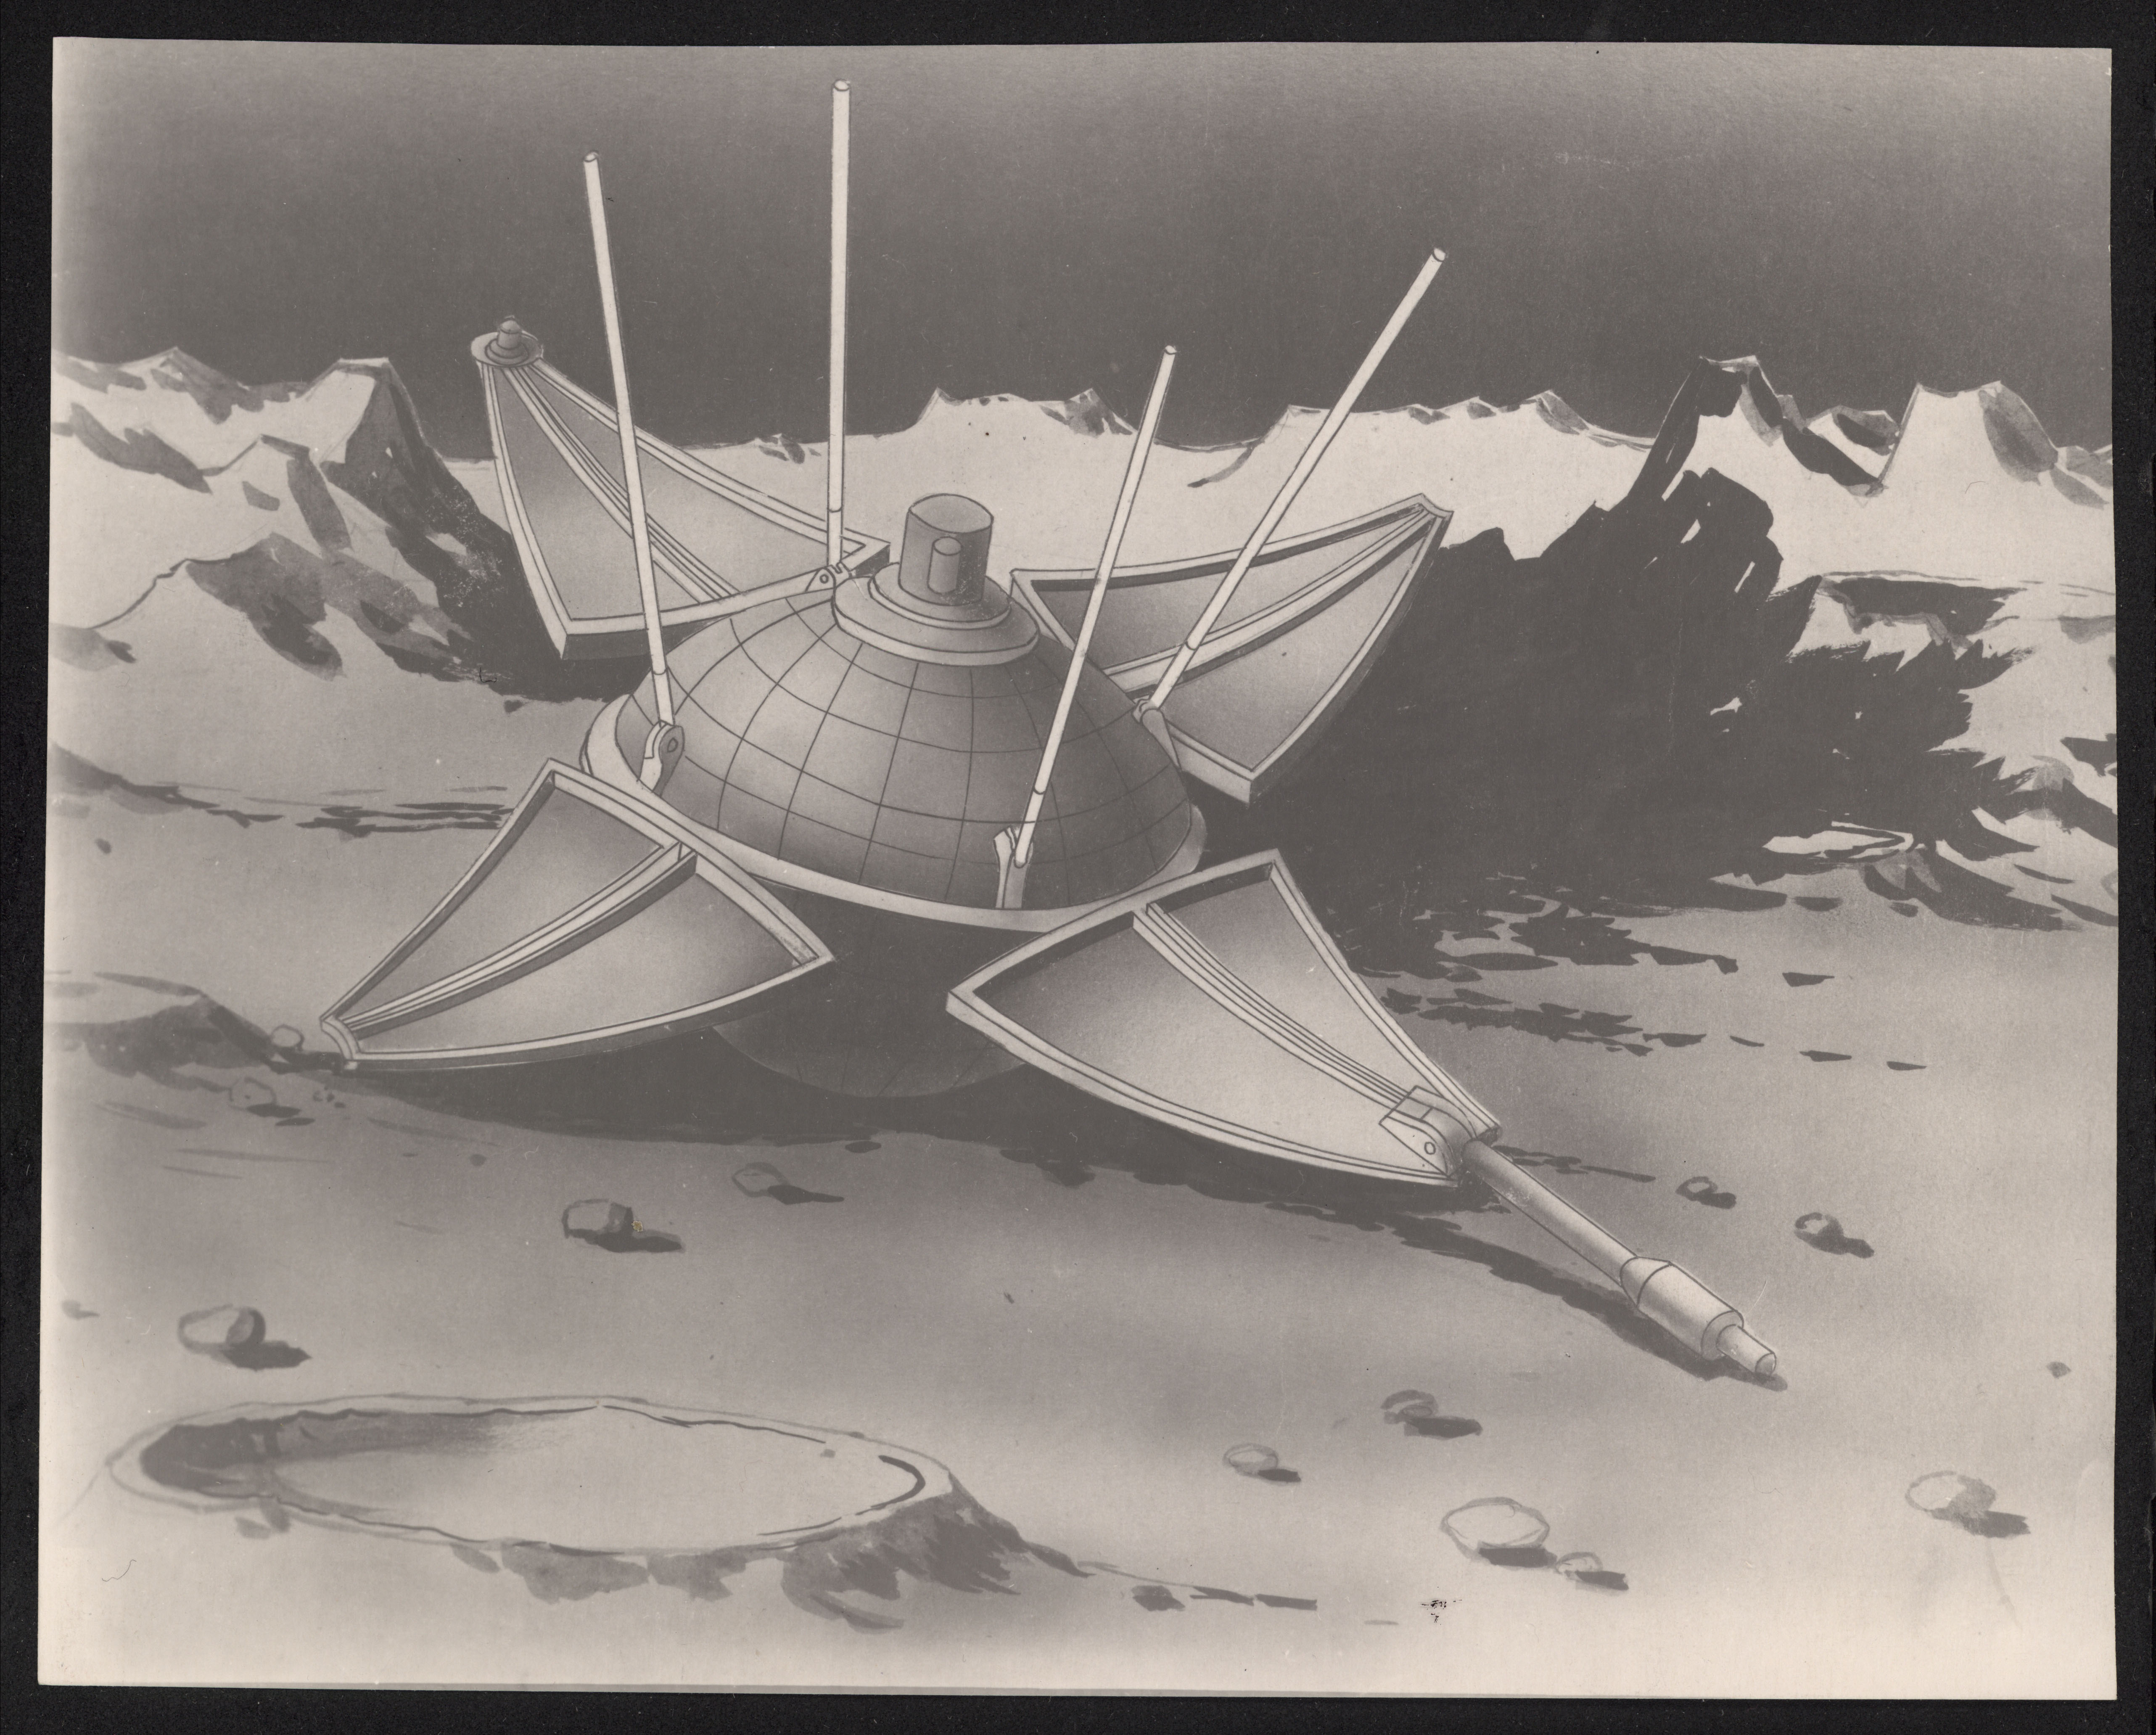
\includegraphics[width=0.4\textwidth]{4164397702}
	\caption{Плакат с художественным изображением автоматической лунной станции <<Луны-9>>}
\end{wrapfigure}

\noindent Подготовка к посадке началась 3 февраля 1966 года за пять часов до достижения цели. Перед торможением станция точно «поймала» лунную вертикаль, а затем, сбросив уже не нужные боковые отсеки, на высоте 75 км от лунной поверхности включила тормозной двигатель. И еще через несколько минут автоматическая лунная станция (АЛС), получившая официальное название, совершила мягкую посадку в точке с координатами 7°8‘ с.ш. и 64°22’ з.д. в районе океана Бурь, западнее кратеров Рейнер и Марий.
\\
\section{Модели}
\subsection{Математическая модель}
 составим ур-е изменение массы со временем, для описания того как изменяется скорость в каждый конкретный промежуток времени будем использовать ур-е циалковсккого, для описания движения самого тела будем использовать второй закон Ньютона
\subsection{Физическая модель}

\section{Программная реализация}

\section{Симуляция}

\section{Медиа}

\section*{Заключение}

\section*{Источники}
\begin{enumerate}
	\item \href{https://ru.wikipedia.org/wiki/%D0%9B%D1%83%D0%BD%D0%B0-9}{Луна-9 - Википедия: для описания миссии и исторической справки}
	\item \href{https://www.roscosmos.ru/29868/#1}{<<Есть мягкая посадка на Луну!>> - статья на странице Роскосмоса}
	\item \href{https://sites.google.com/view/kspmath/home}{The Kerbal Math and Physics Lab}
	\item \href{https://kerbalx.com/}{KerbalX - библиотека воздушных судов в KSP}
\end{enumerate}

\end{document}